\RequirePackage{plautopatch}

\documentclass[gutter=20mm,fore-edge=20mm,head_space=30mm,foot_space=30mm]{jlreq}

% 数式
\usepackage{amsmath,amsfonts,amssymb}
\usepackage{bm}
% 画像
\usepackage[dvipdfmx]{graphicx}

\usepackage{url}
\usepackage[english]{babel}
\usepackage{wrapfig}
\usepackage{float}

\usepackage{siunitx}
\usepackage{enumerate}
\usepackage{enumitem}
\usepackage{multirow}
\usepackage{caption}
\usepackage{listings,jvlisting} %日本語のコメントアウトをする場合jvlisting(もしくはjlisting)が必要
%ここからソースコードの表示に関する設定
\lstset{
  basicstyle={\ttfamily},
  identifierstyle={\small},
  commentstyle={\smallitshape},
  keywordstyle={\small\bfseries},
  ndkeywordstyle={\small},
  stringstyle={\small\ttfamily},
  frame={tb},
  breaklines=true,
  columns=[l]{fullflexible},
  numbers=left,
  xrightmargin=0zw,
  xleftmargin=3zw,
  numberstyle={\scriptsize},
  stepnumber=1,
  numbersep=1zw,
  lineskip=-0.5ex
}



\makeatletter
\newcommand{\figcaption}[1]{\def\@captype{figure}\caption{#1}}
\newcommand{\tblcaption}[1]{\def\@captype{table}\caption{#1}}
\makeatother
\pagestyle{plain}

\title{数値解析レポートNo.3}
\author{4年39番 湯嶋 皓騎}
\date{\number\year{}年\number\month{}月\number\day{}日}

\begin{document}
\newcommand*{\mathun}[1]{{\,\mathrm{[#1]}}}
\newcommand*{\textun}[1]{$\mathun{#1}$}
\renewcommand{\figurename}{Fig. }
\renewcommand{\refname}{参考文献}
\maketitle

\section{指数近似}
式 (\ref{eq:data1}) のデータを式 (\ref{eq:expapprox}) の式を用いて指数近似を行い,結果のグラフを示せ.

\begin{equation}
  (x, y) = (1.5, 8.96),\ (2.0, 14.78),\ (2.5, 24.36),\ (3.0, 40.17) \label{eq:data1}
\end{equation}

\begin{equation}
  y = a_0 e^{a_1 x} \label{eq:expapprox}
\end{equation}

式 (\ref{eq:expapprox}) の両辺の対数を取ると,式 (\ref{eq:logapprox}) のようになる.
\begin{equation}
  \ln y = \ln a_0 + a_1 x \label{eq:logapprox}
\end{equation}
右辺が線形となるため,課題8で用いた線形近似のアルゴリズムを用いて指数近似を行うことができる.

プログラムを List.~\ref{lst:expapprox} に示す.

\begin{lstlisting}[caption=指数近似,label=lst:expapprox]
  Vector *exponentialApproximation(const Matrix *coordinates) {
    size_t param_num = 2;  // a0, a1
    Vector *vector = allocVector(param_num);
    SquareMatrix *matrix = allocSquareMatrix(param_num);
    size_t i, j, k;

    for (i = 0; i < vector->length; i++) {
        for (j = 0; j < coordinates->row; j++) {
            // log(y_i) = log(a0_i) + a1_i x^i
            vector->data[i] += log(coordinates->data[j][1]) *
                               power(coordinates->data[j][0], i);
        }
    }

    for (i = 0; i < matrix->size; i++) {
        for (j = i; j < matrix->size; j++) {
            for (k = 0; k < coordinates->row; k++) {
                matrix->data[i][j] += power(coordinates->data[k][0], i + j);
            }
            matrix->data[j][i] = matrix->data[i][j];
        }
    }

    return solveLinearEquation(matrix, vector);
}  
\end{lstlisting}

ただし,\verb|solveLinearEquation| は引数の行列とベクトルの線形方程式を解いた結果を返す関数であり,
\verb|power(double, size_t)| は引数の値を第二引数の値乗した値を返す関数である.
また,解いた結果のベクトルの第一要素が $\log(a_0)$,第二要素が $a_1$ となる.第一要素が対数になるのは,はじめに対数を取ったためである.

これを実行した結果,$a_0 \approx 1.96, a_1 \approx 1.01$ が得られた.この結果を用いて指数近似を行った結果を Fig.~\ref{fig:expapprox} に示す.

\begin{figure}[H]
  \centering
  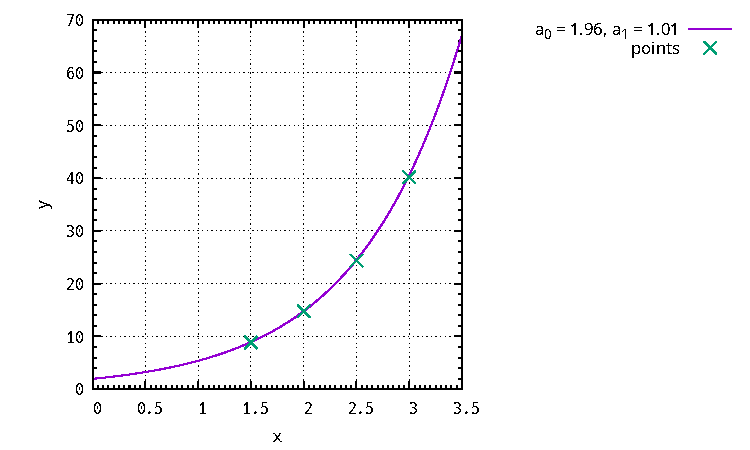
\includegraphics[width=0.8\linewidth]{1/expapprox.pdf}
  \caption{指数近似の結果}
  \label{fig:expapprox}
\end{figure}

Fig.~\ref{fig:expapprox} より,正しく指数近似がなされていそうだとわかる.

\section{これまでに行った相互評価について}
これまでに行った相互評価について述べる.
\subsection{良いと思うところ,参考になったところ}
相互評価を行うことで,プログラムをどのように改善すればよいか,どのような点をアドバイスすればよいかがわかった.
例えばプログラムの動作に問題がある場合,なぜ問題が起きているのか,どのように改善すれば解決するのかをフィードバックとして伝えることができた.

また,相互評価と直接関係することではないが,Windows とそれ以外の Unix 系OS での動作の違いについても知ることができた.
具体的には,\verb|size_t| 型の変数を printf で出力する際に,
Unix 系OS では \%lu もしくは \%zu と指定するが,Windows では \%Iu と指定しないと警告が表示されることがわかった.


\subsection{改善すべきところ,改善案,バグ報告}
\subsubsection{プログラムの入力について}
最初の講義で「入力はcsvファイルのみとする」とアナウンスされていたにも関わらず,ファイル名やパラメータを対話的に入力させるプログラムが散見
された.あまり本質的な問題ではないが,入力方法が統一されていないと相互評価がしにくいため,統一できるようにしたかった.


\subsubsection{プログラムの品質について}
未使用の変数がそのまま残っている,変数名が不適切,動的に確保した領域を解放し忘れているプログラムが多く見られた.
未使用の変数に関してはコンパイラの警告レベルを上げることで解決できるので,提出前にコンパイラの警告レベルを上げた状態でコンパイルが通ることを確認するよう
アナウンスして欲しい.gcc なら \verb|-Wall -Wextra -Werror| オプションを,bcc32c なら \verb|-Weverything -Werror|を付加することで
多くの警告をエラーとして扱うことができ,プログラムの品質を上げることができる.
さらに,gcc なら \verb|-fanalyzer| オプションをつけると,簡単に静的解析ができるので,これもアナウンスして欲しい.

\subsubsection{相互評価の相手について}
同じ人と思われるプログラムが5回中3回の割合で回ってきたので,もう少し他の人のプログラムも評価したかった.

\section{非線形関数に対する数値積分法}
解析的に解ける非線形関数に対して台形・シンプソン・ロンバーグの3手法による数値積分し,それぞれの分割数と誤差,及び
計算量・計算速度について調査する.

\subsection{調査プログラム}
調査プログラムを List.~\ref{lst:integral} に示す.

\begin{lstlisting}[caption=調査プログラム,label=lst:integral]
#include <math.h>
#include <stdbool.h>
#include <stdio.h>
#include <stdlib.h>

#include "NAbasic.h"

#define ROMBERG_TABLE_MAX 255
#define EPS 1e-7

typedef double (*func_t)(double);

void dump_romberg_table(size_t n, size_t p, Vector **T, size_t len) {
    size_t i, j;
    printf("division_num:%zu dimension:%zu\n", n, p);
    puts("Romberg Table");
    for (i = 0; i < len; i++) {
        for (j = 0; j < T[i]->length; j++) {
            printf("%.10f  ", T[i]->data[j]);
        }
        putchar('\n');
    }
}

double trapezoid(func_t f, double a, double b, size_t n) {
    double h = (b - a) / n;
    double sum = 0.0;
    size_t i;

    // sum = h*(f(a)/2 + f(a + h) + f(a + 2h) + ... + f(a + (n - 1)h) + f(b)/2)
    // where (a + nh = b)
    for (i = 1; i < n; i++) sum += f(a + i * h);
    sum += (f(a) + f(b)) / 2.0;

    return h * sum;
}

double simpson(func_t f, double a, double b, size_t n) {
    double h = (b - a) / 2.0 / n;
    double sum = 0.0;
    size_t i;

    // sum = h*(f(a) + 4*f(a + h) + 2*f(a + 2h) + ...  + f(b)/6)/3.0
    for (i = 1; i < 2 * n; i++) {
        size_t power = (i % 2 == 0) ? 2 : 4;
        sum += f(a + i * h) * power;
    }
    sum += f(a) + f(b);

    return h * sum / 3.0;
}

double romberg(func_t f, double a1, double a2, size_t k_max) {
    size_t i, k, m = 1;
    size_t n = 1, p = 1;  // n = 2^k, p = 4^m
    double result;
    Vector **T;
    bool is_converged = false;

    // T を長さ k_max で確保し,T[0] は長さ 1 で確保する

    T[0]->data[0] = (a2 - a1) * (f(a1) + f(a2)) / 2.0;

    for (k = 1; ((k < k_max) && !(is_converged)); k++) {
        double h, sum = 0.0;

        // T[k] を長さ k+1 で確保

        n *= 2;  // n = 2^k
        h = (a2 - a1) / n;
        // sum = f(a + h) + f(a + 3h) + ... + f(a+(2n-1)h)
        for (i = 1; i < n; i += 2) sum += f(a1 + i * h);
        // T[k][0] = T[k-1][0]/2 + h*sum (k >= 1)
        T[k]->data[0] = T[k - 1]->data[0] / 2 + h * sum;

        for (m = p = 1; m <= k; m++) {
            p *= 2;  // p = 2^m
            // T[k][m] = T[k][m-1] + (T[k][m-1] - T[k-1][m-1])/(p^2-1) (k >= 1)
            T[k]->data[m] =
                T[k]->data[m - 1] +
                (T[k]->data[m - 1] - T[k - 1]->data[m - 1]) / (p * p - 1);
            if (fabs(T[k]->data[m] - T[k - 1]->data[m - 1]) < EPS) {
                T[k]->length = m + 1;
                is_converged = true;
                break;
            }
        }
    }

    result = T[k - 1]->data[m - 1];
    for (i = 0; i < k; i++) freeVector(T[i]);
    free(T);

    return result;
}

int main(void) {
    double res;
    double x_s = 0, x_e = 3;
    size_t n;
    func_t f = exp;
    double exact_value;

    printf("Trapezoid\n");
    for (n = 1; n <= 1000; n++) {
        res = trapezoid(f, x_s, x_e, n);
        printf("%zu,%.10f,%.10f\n", n, res, (res - exact_value));
    }

    printf("Simpson\n");
    for (n = 1; n <= 1000; n++) {
        res = simpson(f, x_s, x_e, n);
        printf("%zu,%.10f,%.10f\n", n, res, (res - exact_value));
    }

    printf("Romberg\n");
    for (n = 1; n <= 10; n++) {
        res = romberg(f, x_s, x_e, n);
        printf("%zu,%.10f,%.10f\n", n, res, (res - exact_value));
    }
    return EXIT_SUCCESS;
}
\end{lstlisting}

変数 \verb|x_s|, \verb|x_e| に積分範囲の始点と終点,\verb|exact_value|に解析解の値を,
\verb|f| に積分する関数を指定する.

\subsection{分割数と誤差}
典型的な非線形関数である指数関数と周期関数である三角関数に対して台形・シンプソン・ロンバーグの3手法による数値積分を行い,
分割数と誤差の関係を調査する.

\subsubsection{指数関数}
指数関数 $f(x) = e^x$ に対して,台形・シンプソン・ロンバーグの3手法による数値積分を行った.
積分範囲は $[0, 3]$ とする.

まず,解析解は
\begin{equation}
  \int_0^3 e^x dx = e^3 - 1 \approx 19.08553692
\end{equation}
である.

次に数値積分の分割数対誤差のグラフを Fig.~\ref{fig:exp} に示す.両対数グラフであることに注意すること.

\begin{figure}[H]
  \centering
  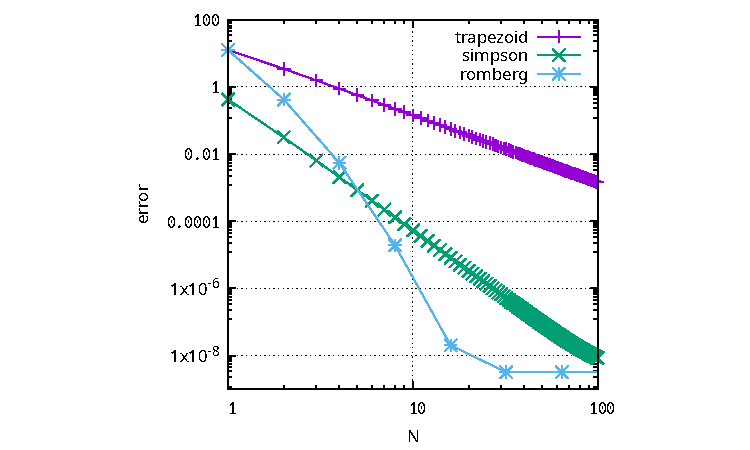
\includegraphics[width=0.8\linewidth]{3/exp/exp.pdf}
  \caption{指数関数に対する数値積分の分割数対誤差}
  \label{fig:exp}
\end{figure}

ただし,ロンバーグ法では分割数32,補間次数16でステップ間誤差が $10^{-7}$ 以下になるため,実際には
分割数32以降は計算を行っていない.

Fig.~\ref{fig:exp} を見ると,台形法とシンプソン法は傾きがほぼ一定だから
分割数と誤差の関係は羃関数的であることがわかる.台形法の傾きは $-2$,シンプソン法の傾きは $-4$ だから,
台形法の誤差は $O(N^2)$,シンプソン法の誤差は $O(N^4)$の速さで小さくなることがわかる.
一方,ロンバーグ法は羃関数的ではなく,他の二つの手法と比べて$N=8$以上で小さい誤差が得られており,
$N=32$でステップ間誤差が $10^{-7}$ 以下になるため,計算を打ち切り,その時点での絶対誤差は$10^{-9}$オーダー
である.

\subsubsection{三角関数}
三角関数 $f(x) = \sin x$ に対して,台形・シンプソン・ロンバーグの3手法による数値積分を行った.
積分範囲は $[0, \pi/2]$ とする.ここで,\verb|PI|$=3.14159265358979323846$とした.

まず,解析解は
\begin{equation}
  \int_0^{\pi/2} \sin x dx = 1
\end{equation}
である.

次に数値積分の分割数対誤差のグラフを Fig.~\ref{fig:sin} に示す.両対数グラフであることに注意すること.

\begin{figure}[H]
  \centering
  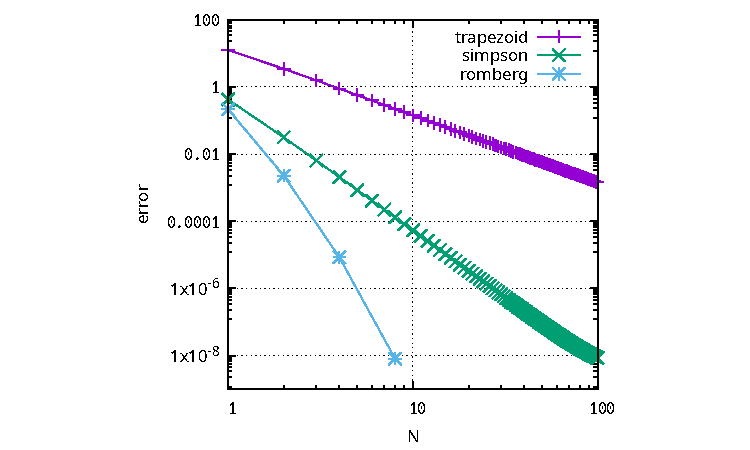
\includegraphics[width=0.8\linewidth]{3/sin/sin.pdf}
  \caption{三角関数に対する数値積分の分割数対誤差}
  \label{fig:sin}
\end{figure}

Fig.~\ref{fig:sin} より,台形法の誤差は$O(h^2)$,シンプソン法は$O(h^4)$であることが再確認できる.
また,ロンバーグ法は$N=16$で誤差が0になってしまったため,それ以降はグラフ上に描画されていない.

\subsubsection{まとめ}
台形法の誤差は$O(N^2)$,シンプソン法は$O(N^4)$の速さで小さくなり,また
いずれの場合においても,ロンバーグ法は他の二つの手法と比べてより早く誤差の小さな値を得ることができることがわかった.

\subsection{計算量・計算速度}
台形・シンプソン・ロンバーグの3手法における計算量と計算速度について調査する.

\subsubsection{計算量}
分割数を$N$として,台形法とシンプソン法の計算量は$O(N)$であり,ロンバーグ法の計算量は$O(N^2)$である.
これは関数の入れ子になっているforループの最大値を数えることでわかる.

\subsubsection{計算速度}
一見すると計算量が$O(N^2)$であるロンバーグ法が遅いように見えるが,前述の通り
ロンバーグ法は収束が速いため,実際には台形法やシンプソン法よりも早く収束した.そのため,
今回のケースではロンバーグ法を用いることが最も効率的であると言える.
しかし,ロンバーグ法は補外を用いて漸化的に精度を上げていくため,処理の並列化が困難である.一方,
台形法やシンプソン法は互いの計算が独立であるため,並列化が容易である.そのため,非常に広い範囲の
数値積分を行う場合には,ロンバーグ法よりも台形法やシンプソン法を用いることが望ましいだろう.

\section{感想}
今回のレポート執筆を通して講義で学んだ内容を復習することで,数値積分法についての理解が深まった.
今後は演習を行った数値積分法以外のアルゴリズムについても調査していきたい.

\begin{thebibliography}{99}
\bibitem{bcc32c} Embarcadero C++ Compiler Warnings: \url{https://docwiki.embarcadero.com/RADStudio/Sydney/en/C%2B%2B_Compiler_Warnings}
\end{thebibliography}

\end{document}
